% NOTE: all of this content has been moved to irt_background and knowledge_tracing_background
\chapter{Survey of Relevant Neural Networks}

In recent years, artificial neural networks (ANN) have become an increasingly popular tool for machine learning problems. Though they have been around since the 1960's \cite{rosenblatt1961}, GPU technology has become more accessible and modern computers are more powerful, allowing anyone interested to train a basic neural network on their machine. ANN can be applied to a diverse set of problems, including regression, classification, computer vision, natural language processing, function approximation, data generation, and more \cite{hammerstrom1993} \cite{zhang2000}.

One of the biggest critiques of ANN is their black-box nature, meaning that the decision process that a trained model uses is typically not explainable by humans. As opposed to simpler methods such as decision trees or linear regression, neural networks are not interpretable. This makes them less desirable in certain applications where researchers wish to know \textit{why} a model predicts a particular data sample the way that it does. For example, if a financial institution is using data-driven methods to determine whether or not to approve someone's loan, the institution should be able to explain to the customer why they were denied. Most customers will not be satisfied with ``the computer told us so,'' and it is possible that a black-box neural network could learn and use sensitive information such as race, age, or gender in its prediction, which would raise legal questions in the United States \cite{ecoa}.

The push for explainable AI has led to multiple approaches to increase model interpretability. Some have aimed to incorporate deep learning methods with existing interpretable methods, in hopes of increasing the performance of explainable methods without sacrificing its interpretability \cite{goebel2018}. Another option is to use a sort of hybrid learning, where interpretable models defer to a black-box model if they are not confident in their prediction \cite{rafique2020}. Others have started with deep models and cut back on complexity, making specific modifications which increase interpretability. For example, the loss function of a convolutional neural network can be adapted so that humans can understand the features extracted in the hidden layers \cite{zhang2018interpretable}. 

The field of education is an application which often desires interpretable models. Researchers often need to be able to point out specific details of decisions made by AI. A student deserves an answer to \textit{why} they failed a test, and a teacher should be given instructions on \textit{how} to fix the student's misconceptions.

\section{Autoencoders}
An autoencoder (AE) is a neural network where the input and output layers are the same shape. The objective for a given data point is to minimize the difference between the output, called the reconstruction, and the input. Typically, the middle hidden layers of an AE are of smaller dimension than the input space. In this way, autoencoders are an unsupervised learning technique for (nonlinear) dimension reduction. Mathematically, we can define an autoencoder in two parts as follows.

For an input $x \in \R^n$, define the \textit{encoder} as a function $f: \R^n \to \R^m$ mapping $x \mapsto z := f(x)$. Usually, $m < n$, and $z$ lies in a hidden feature space. The encoder sends an observed data point to its representation in a learned feature space. Define the \textit{decoder} as a function $g: \R^m \to \R^n$ mapping $z \mapsto \hat x := g(z)$. The decoder maps a hidden representation $z$ to a reconstruction of the encoder input. Note that in our case, the functions $f$ and $g$ are both parameterized by neural networks, each of which can have any number of hidden layers. The end-to-end autoencoder is then the function composition $\mathcal{A}(x):= g(f(x)): \R^n \to \R^n$. To train an AE, the loss function minimizes the difference between the input and output. This can be done in a number of ways, including the simple mean squared error loss
\begin{equation}
  \mathcal{L}(x) = || x - g(f(x))||_2^2
  \label{eq:mse}
\end{equation}
or cross-entropy loss for binary data
\begin{equation}
  \mathcal{L}(x) = \sum_{i=1}^n - x_i \log(g(f(x_i))) - (1-x_i)\log(1- g(f(x_i))).
  \label{eq:cross_entropy}
\end{equation}

Autoencoders with only a single hidden layer can be compared with nonlinear principal components analysis (PCA), and using linear activation functions allows for recovery of PCA loading vectors \cite{plaut2018}. AEs have clear applications in image compression straight out-of-the-box, and can be modified for more complicated problems. Denoising autoencoders \cite{vincent2008} are capable of processing noisy images and cleaning them up. To do this, they corrupt input data by deleting pixels at random and reconstructing the original image. Autoencoders can also be modified for data generation applications using a variational autoencoder.

\section{Variational Autoencoders}
\sideremark{could include citations: infoVAE, ELBO, ``towards deeper understanding of VAE''}

% could talk about how Zhao et al (InfoVAE) show that if decoder is Gaussian, then maximizing ELBO makes the latent distribution bad - but I've shown this isn't the case in our model, where the decoder is Bernoulli.

The motivation for designing a variational autoencoder (VAE), introduced by Kingma and Welling \cite{kingma2014}, is different from regular autoencoders in that it is not rooted in neural networks. Rather, a probabilistic point of view provides the main source of motivation, and neural networks are a very common tool used to implement a VAE.

Consider a dataset $\mathbb{X} = \{\vect x_i\}_{i=1}^N$, where each data point $\vect x_i \in \R^n$ is generated by a random process involving an unobserved variable $\vect z \in \R^d$. This unobserved variable is often referred to as ``latent code.'' It is assumed that to generate the observed data point $\vect x_i$, a value $\vect z_i$ is first sampled from a prior distribution $p_*(\vect z)$, and then $x_i$ is generated from a distribution $p_*(\vect x | \vect z)$.

From observing the dataset $\mathbb{X}$, the latent variables $\vect z_i$ and parameters of the distributions $p_*(\vect z)$ and $p_*(\vect x | \vect z)$ are unknown. The goal of a VAE is to approximate these values, which leads to the ability to represent/encode data and generate new data. This should be done with a general algorithm that is unaffected by (i) intractability of the marginal likelihood $p(\vect x) = \int p(\vect z) p(\vect x | \vect z) d\vect z$ and (ii) large amounts of data. \sideremark{maybe point out this is a common problem with IRT param est methods} Note that (i) is important because if $p(\vect x)$ is intractable and thus $p(\vect z | \vect x)$ is intractable, then the EM algorithm cannot be used.

In order to implement this task, two neural networks $q_\alpha(\vect z | \vect x)$ and $p_\beta(\vect x | \vect z)$ (probabilistic encoder and decoder, respectively) are used to approximate the unobservable true posterior distributions $p_{\alpha^*}(\vect z| \vect x)$ and $p_{\beta^*}(\vect x | \vect z)$. In the encoder/decoder, the indices $\alpha$ and $\beta$ reference settings of the trainable parameters of the neural network. Note that unlike a regular autoencoder, the probabilistic encoder $q_\alpha(\vect z | \vect x)$ of a VAE outputs a probability distribution for $\vect z$ given $\vect x$, rather than a single value.

\subsection{A note on Information Theory}
Before continuing, we introduce some ideas from information theory: entropy, cross-entropy, and KL-Divergence \cite{pattern_rec_book}. Consider a random variable $x$. For a particular value $x_0$, we can compute the amount of information gained from observing $x_0$ as $h(x_0) = -\log_2 p(x=x_0)$. When we use $\log_2$, the unit for information is ``bits,'' but any logarithm can be used. Note that we gain more information from observing a low-probability event than from observing a high-probability event. 

\textit{Entropy} is defined as the expectation of $h(x)$: the average amount of information that will be learned by observing a random $x$. So the entropy of the random variable $x$ is given as 
\begin{equation}
  H[p] = - \int p(x) \log p(x)dx
  \label{eq:entropy}
\end{equation}

Now assume that we also have access to a distribution $q(x)$ which approximates a possibly unknown $p(x)$. \textit{Cross-entropy} is the average amount of information needed to identify an event $x$ which was drawn from $q$ instead of $p$. Cross-entropy is given as
\begin{equation}
  H[p,q] = - \int p(x) \log q(x) dx
  \label{eq:xentropy}
\end{equation}

We can simply define \textit{Kullback-Leibler Divergence} (KL-Divergence) \cite{kullback1951} as 
\begin{equation}
  \mathcal{D}_{KL}\left[ p || q \right] = H[p] - H[p,q] = - \int p(x) \log \left(\frac{q(x)}{p(x)} \right)dx
  \label{eq:kl_div}
\end{equation}
Intuitively, KL-Divergence is amount of information which is lost if the approximating distribution $q(x)$ is used instead of the true distribution $p(x)$. However, KL-Divergence cannot be interpreted as a metric or as a distance between $p$ and $q$ because it is not symmetric -- in general, $\mathcal{D}_{KL}[p||q] \not = \mathcal{D}_{KL}[q||p]$. KL-Divergence is non-negative, and $\mathcal{D}_{KL}[p||q] = 0$ iff $p(x) = q(x)$.

\subsection{VAE Derivation}\label{sec:vae_derive}

We derive the desired loss function for a VAE. The log marginal likelihood is given as
\begin{equation}
  \log p_{\beta}(\vect x_1,\ldots,\vect x_N) = \sum_{i=1}^N \log p_{\beta}(\vect x_i)
  \label{eq:vae_marginal}
\end{equation}
Denoting $\vect x = \vect x_i$, we can rewrite each $p_{\beta}(\vect x_i)$ as \sideremark{I don't know the best way to index $p_\beta$ }
\begin{equation}
  \begin{split}
    \log p_{\beta}(\vect x) &= \int q_\alpha(\vect z |\vect x) \log p_{\beta} (\vect x)d\vect z \\
    &= \int q_\alpha(\vect z | \vect x) \log \left( \frac{p_{\beta}(\vect z | \vect x) p_{\beta}(\vect x)}{p_{\beta}(\vect z | \vect x)} d\vect z \right) \\
    &= \int q_\alpha(\vect z | \vect x) \log \left( \frac{p_{\beta}(\vect x, \vect z)}{p_{\beta}(\vect z | \vect x)} \right) d\vect z\\
    &= \int q_\alpha(\vect z | \vect x) \left( \log \frac{q_\alpha(\vect z | \vect x)}{p_{\beta}(\vect z | \vect x)} + \log \frac{p_{\beta}(\vect x, \vect z)}{q_\alpha(\vect z | \vect x)}\right) d\vect z \\
    &= \mathcal{D}_{KL}\left[ q_\alpha(\vect z |\vect x) || p_{\beta}(\vect z | \vect x) \right] + \int q_\alpha(\vect z | \vect x) \log \left( \frac{p_{\beta}(\vect x, \vect z)}{q_\alpha(\vect z | \vect x)} \right)d\vect z \\
    &= \mathcal{D}_{KL}\left[ q_\alpha(\vect z |\vect x) || p_{\beta}(\vect z | \vect x) \right] + \mathbb{E}_{q_\alpha(\vect z | \vect x)}\left[ -\log q_\alpha(\vect z | \vect x) + \log p_{\beta}(\vect x, \vect z) \right] \\
    &= \mathcal{D}_{KL}\left[ q_\alpha(\vect z |\vect x) || p_{\beta}(\vect z | \vect x) \right] + \tilde{\mathcal{L}}(\alpha, \beta; \vect x)
\label{eq:vae_derive}
  \end{split}
\end{equation}

Note that in the final line, the first term is the KL-Divergence between the approximate and true posterior. Since we don't know the true posterior, we can't calculate this term. But notice that since KL-Divergence is always positive, and we can write 
\begin{equation}
  \begin{split}
    \log p_\beta (\vect x) \geq \tilde{\mathcal{L}}(\alpha, \beta; \vect x) = -\mathcal{D}_{KL}\left[ q_\alpha(\vect z | \vect x) || p_{\beta}(\vect z) \right] + \mathbb{E}_{q_\alpha(\vect z | \vect x)}\left[ \log p_{\beta}(\vect x | \vect z) \right]
  \label{eq:elbo}
\end{split}
\end{equation}

The term $\tilde{\mathcal{L}}(\alpha, \beta; \vect x)$ is referred to as the variational lower bound or Evidence Lower Bound (ELBO). Increasing the ELBO by varying the parameters $\alpha$ and $\beta$ will increase the marginal likelihood $\log p_\beta(\vect x)$, even though we ignore the term $\mathcal{D}_{KL}\left[ q_\alpha (\vect z | \vect x) || p_\beta(\vect z | \vect x) \right]$.

We take the ELBO $\tilde{\mathcal{L}}(\alpha,\beta; \vect x)$ to be a potential VAE objective function which we want to maximize. In Equation \ref{eq:elbo}, the first term gives the negative KL-Divergence between the probabilistic encoder $q_\alpha(\vect z | \vect x)$ and the true prior distribution of the latent code $p_\beta(\vect z)$. Note that unlike the true posterior $p_\beta(\vect z | \vect x)$, the true prior is known and is nearly always assumed to be independent Gaussian. 

For now, we assume that $\vect z \sim \mathcal{N}(0,I)$. Additionally, we assume that the encoder outputs a standard normal distribution. In Section \ref{sec:cov}, we propose architecture which fits the assumption that $\vect z \sim \mathcal{N}(\mu, \Sigma)$ and allows for the encoder to output a multivariate Gaussian distribution.

These assumptions make computing $\tilde{\mathcal{L}}(\alpha,\beta;\vect x)$ much easier. It can be shown \cite{doersch2016} that \sideremark{Should I show this?} the KL-Divergence between an independent Gaussian distribution and a standard normal distribution of dimension $K$ is calculated as
\begin{equation}
  \mathcal{D}_{KL}\left[ \mathcal{N}(\vect \mu_0, \vect \sigma_0^2I) || \mathcal{N}(0,I) \right] = \frac{1}{2}\sum_{k=1}^K \left( \mu_k^2 + \sigma_{0,k}^2 - 1 - \log(\sigma_{0,k}^2)\right)
  \label{eq:ind_gauss_kl}
\end{equation}
Note that the vectors $\vect \mu_0$ and $\vect \sigma_0^2$ are outputted by the encoder $q_\alpha(\vect z | \vect x_0)$, given the observed input $\vect x_0$. Since Equation \ref{eq:ind_gauss_kl} is in closed form, there is no difficulty in calculating the (possibly high-dimensional) integral that is usually required to compute KL-Divergence.

The second term in Equation \ref{eq:elbo} is similar to Equation \ref{eq:xentropy}, and depends on the probabilistic decoder $p_\beta(\vect x | \vect z)$, which is usually assumed to be either Gaussian or Bernoulli. Considering the desired application of educational measurement where data is given as binary responses, we assume that the decoder is Bernoulli. To deal with the expectation over $q_\alpha$, we simply sample $L$ times from $q_\alpha(\vect z | \vect x)$. In practice, it is often simplest to just choose $L=1$ \cite{kingma2014}. So then 
\begin{equation}
  \begin{split}
    \mathbb{E}_{q_\alpha(\vect z | \vect x)} \left[ \log p_\beta(\vect x | \vect z) \right] &\approx \frac{1}{L}\sum_{l=1}^L \log p_\beta(\vect x | \vect z^{(l)}) \\
    &\approx \log p_\beta(\vect x| \vect z^*) \\
    &= \log\left( \prod_{i=1}^n p_\beta(x_i = 1 | \vect z^*)^{x_i} \cdot p_\beta(x_i=0 | \vect z^*)^{x_i} \right) \\
  &= \sum_{i=1}^n x_i\log \hat x_i + (1-x_i)\log (1-\hat x_i)
  \end{split}
  \label{eq:bernoulli}
\end{equation}
where $\hat x_i = p_\beta(x_i=1 | \vect z^*)$ gives $\hat{\vect x} = \{\hat x_i\}_{i=1}^n$, the reconstruction of the input $\vect x$ from the encoder $q_\alpha$. Note that the final line of Equation \ref{eq:bernoulli} results in the negative binary cross-entropy loss function commonly used in classification problems.

The process is summarized as follows: given an input vector $\vect x_0 \in \R^n$, we obtain the posterior distribution $q_\alpha(\vect z | \vect x_0)$ (this is done by feeding $\vect x_0$ through a neural network). Sample $\vect z^* \sim q_\alpha(\vect z |\vect x_0)$, and compute $\hat{\vect x} = p_\beta(\vect x | \vect z^*)$ (this is done by feeding $\vect z^*$ through a neural network). As demonstrated in Equation \ref{eq:ind_gauss_kl} and Equation \ref{eq:bernoulli}, we can easily compute the objective function $\tilde{\mathcal{L}}(\alpha, \beta; \vect x_0)$.

Usually when working with neural networks, goal is to minimize an loss function, rather than maximize an objective function. As such, we define the loss function 
\begin{equation}
  \label{eq:vae_loss}
  \begin{split}
  \mathcal{L}&(\alpha, \beta; \vect x) = - \tilde{\mathcal{L}}(\alpha, \beta;\vect x) \\
  &= \Big(\sum_{i=1}^n - x_i\log p_\beta(x_i | \vect z^*) - (1-x_i)\log (1-p_\beta(x_i | \vect z^*)) \Big) + \mathcal{D}_{KL}\left[ q_\alpha(\vect z | \vect x) || p_\beta(\vect z) \right]
  \end{split}
\end{equation}
where $\vect z^* \sim p_\beta(\vect z) = \mathcal{N}(0,I)$. The parameters $\alpha$ and $\beta$ represent the weights and biases of the encoder and decoder, and are updated via a gradient descent algorithm in order to minimize Equation \ref{eq:vae_loss}. Note that $\mathcal{L}(\alpha, \beta; \vect x)$ can simply be understood as reconstructing a binary input $\vect x$ via the first term, while regularizing on the latent code via the second term.


\subsection{Implementation Details}
Recall that each observed data point $\vect x_i \in \R^n$ and the corresponding latent code $\vect z_i \in \R^d$. To parameterize the encoder $q_\alpha(\vect z | \vect x)$ as a neural network, an input layer with $n$ nodes is required. The encoder can (but does not need to) include a number of hidden layers of varying size. The output of the encoder must include $2\cdot d$ nodes, assuming that $p_\beta(\vect z) = \mathcal{N}(0,I)$. 

Notice that in Equation \ref{eq:ind_gauss_kl}, there is a term $\log(\sigma_{0,k}^2)$, dependent on input $\vect x_0$ and all parameters of the encoder. If at any point during training $\sigma_{0,k}^2 \leq 0$ for any $k$, then the VAE loss would not be possible to calculate. To avoid this issue and ensure that $\sigma_{0,k}^2 > 0$ regardless of inputs or encoder parameters, the encoder outputs the log-variances rather than the variances. The first $d$ nodes outputted by the encoder represent the latent mean vector $\vect \mu$, and the last $d$ nodes represent the $\log$ latent variances $\log \vect \sigma^2$. So for an observed input $\vect x_0$, the encoder will output a $d$-dimensional standard normal distribution $\mathcal{N}(\vect \mu_0, \vect \sigma_0^2I)$.

The input layer of the decoder $p_\beta(\vect x | \vect z)$ has $d$ nodes and takes in a sample from $\mathcal{N}(\vect \mu_0, \vect \sigma_0^2I)$, given the original input $\vect x_0$. But the sampling operation is not differentiable, posing a problem for backpropagation-based gradient descent. A re-parameterization is used: sample $\vect \e_0 \sim \mathcal{N}(0,I)$, then calculate $\vect z_0 = \vect \mu_0 + \vect \e_0 \odot \vect \sigma_0^2$ where $\odot$ is element-wise vector multiplication. Then $\vect z_0$ is fed through an optional number of hidden layers to an output layer of size $n$. The output can be interpreted as a reconstruction $\hat{\vect x_0}$.

\begin{figure}[h]
  \centering
  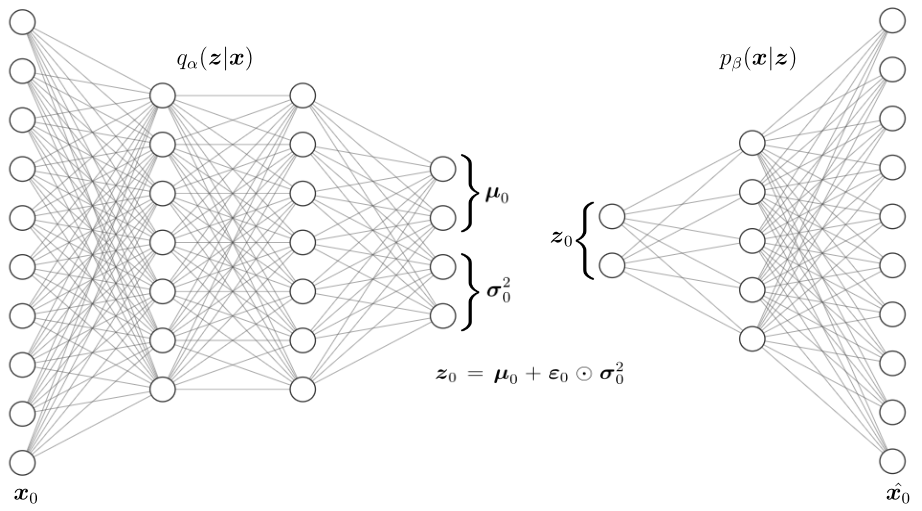
\includegraphics[width=.95\textwidth]{img/vae_visual.png}
  \caption{Visualization of a VAE architecture with $n=10$ and $d=2$.}
  \label{fig:vae_visual}
\end{figure}
The VAE architecture is summarized in Figure \ref{fig:vae_visual}. Note that the VAE does not need to be symmetric; the encoder and decoder can have a different number of hidden layers of different sizes.

\section{Time Series Neural Networks}
In many deep learning applications such as video processing, natural language processing, or dynamical systems, the observed data is time-dependent \cite{kahou2015} \cite{vaswani2017} \cite{gilpin2020}.In such datasets, a single observation of $d$ features can not represented as a vector $\vect x_0 \in \R^d$, but must take into account the $T$ different measurements of the $d$ features, each taken at a different timestep $1 \leq t \leq T$. As such, a data point is represented as a matrix $X_0 \in \R^{d \times T}$, where each column $t$ of $X_0$ gives a snapshot of the observation at time $t$. 

\subsection{Recurrent Neural Networks}
Recurrent Neural Networks (RNN) are the most simple adaptation of neural networks to deal with time-series data. A regular feed-forward neural network layer takes an input vector $\vect x \in \R^d$ and outputs
\begin{equation}
  \vect y = f( W\vect x + \vect b)
  \label{eq:ffn_layer}
\end{equation}
where $W \in \R^{h \times d}$ and $\vect b \in \R^h$ are trainable parameters and $f$ is a non-decreasing activation function \cite{sharma2020}. 

In the time-dependent setting, let $\vect x_t$ be a column of an input $X$. A basic recurrent layer calculates 
\begin{equation}
  \begin{split}
    \vect h_t &= \tanh(W_{hh}\vect h_{t-1} + W_{hx}\vect x_t + \vect b_h) \\
    \vect y_t &= \sigma(W_{hy}[\vect x_t, \vect h_t] + \vect b_y)
\end{split}
  \label{eq:rnn_layer}
\end{equation}
where $W_{hh} \in \R^{h\times h}$, $W_{hx}\in \R^{h\times d}$, $\vect b_h \in \R^h$, $W_{hy} \in \R^{h \times (h+d)}$, and $\vect b_y \in \R^h$ are trainable parameters \cite{elman1990}. The notation $[\vect x_t, \vect h_t]$ refers to vector concatenation. Note that this allows the output $\vect y_t$ to include information from previous time-steps. A visualization of an unfolded RNN is shown in Figure \ref{fig:rnn_visual}.

\begin{figure}[h]
  \centering
  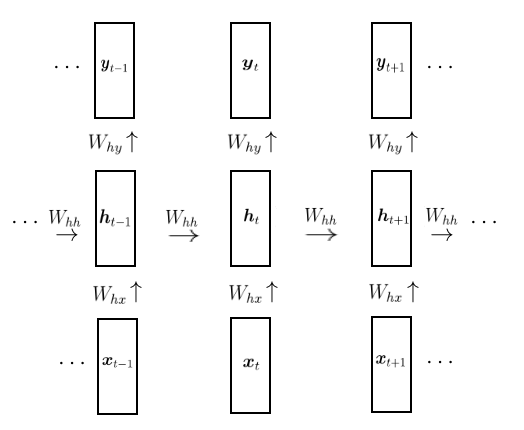
\includegraphics[width=.5\textwidth]{img/rnn_visual.png}
  \caption{Architecture of a recurrent neural network.}
  \label{fig:rnn_visual}
\end{figure}

One issue that RNN face is the exploding or vanishing gradient problem \cite{bengio1994}, where the norm of the gradient can become very large or very small during training. This is due to the fact that partial derivatives calculated during back-propagation between hidden states at time $t_1$ and $t_2$ is found by a product of $t_2 - t_1$ Jacobian matrices \cite{pascanu2013}. As the difference between $t_1$ and $t_2$ increases, the corresponding partial derivatives $\frac{\partial \vect h_{t_1}}{\partial \vect h_{t_2}}$ can exponentially grow or exponentially decay in norm.

Related to the exploding/vanishing gradient issue, RNN experience difficulty in retaining important information for multiple time-steps is difficult. For example, if an important phenomena happens to data point $X_0$ at time $t$, then that information should still influence the values of $\vect h_{t+10}$ and $\vect y_{t+10}$. But the structure described in Equation \ref{eq:rnn_layer} and Figure \ref{fig:rnn_visual} causes the impact of $\vect x_t$ and $\vect h_t$ to fade over time.


\subsection{Long Short-Term Memory Networks}
To combat this issue, Long Short-Term Memory (LSTM) networks were developed by Hochreiter and Schmidhuber \cite{hochreiter1997}. This architecture introduces element-wise multiplication and addition operations in addition to multiple trainable weights matrices which allows for tracking long-term dependencies. An LSTM layer computes a ``cell state'' vector $\vect c_t$, in addition to the hidden layer representation $\vect h_t$. This cell state is updated at each time-step to ``remember'' important information and ``forget'' frivolous information.

The LSTM structure also addresses the exploding/vanishing gradient of RNN. The presence of the cell state $\vect c_t$ ensures that calculating derivatives of long-range dependencies do not include many matrix multiplications \cite{hochreiter1997}.

A single cell of an LSTM can be compared to the middle block in Figure \ref{fig:rnn_visual} containing $\vect h_t$ of an RNN. At time $t$, given an input $t$ $\vect x_t$, previous hidden state $\vect h_{t-1}$, and previous cell state $c_{t-1}$, an LSTM cell uses four trainable weights matrices and four element-wise operations. First compute the ``forget'' vector $\vect f_t$, the ``update'' vector $\vect u_t$, the ``add'' vector $\vect a_t$, and the ``filter'' vector $\vect g_t$.
\begin{equation}
\begin{split}
  \vect f_t &= \sigma(W_f [\vect x_t, \vect h_{t-1}] + \vect b_f) \\
  \vect u_t &= \sigma(W_u [\vect x_t, \vect h_{t-1}] + \vect b_u) \\
  \vect a_t &= \tanh(W_a [\vect x_t, \vect h_{t-1}] + \vect b_a) \\
  \vect g_t &= \sigma(W_g [\vect x_t, \vect h_{t-1}] + \vect b_g)
\end{split}
  \label{eq:lstm_vects}
\end{equation}

The first three vectors in Equation \ref{eq:lstm_vects} are used to perform element-wise operations on $\vect c_{t-1}$ to produce the next cell state $\vect c_t$, and $\vect g_t$ is used in updating $\vect h_t$. Notice that the sigmoid activation function $\sigma(\cdot)$ maps small inputs to near $0$ and large inputs to near $1$, while the hyperbolic tangent activation function $\tanh(\cdot)$ maps small inputs to near $-1$ and large inputs to near $1$. 

Using $\vect f_t$, unimportant aspects (elements near zero) of $\vect c_{t-1}$ are forgotten:
\begin{equation}
  \vect c_{t-1}^* = \vect c_{t-1} \times \vect f_t
  \label{eq:lstm_forget}
\end{equation}
where $\times$ is element-wise multiplication. Next, $\vect u_t$ decides what information to update (elements near one), and $\vect a_t$ gives the value (an increase or decrease) of the information to be updated:
\begin{equation}
  \vect c_t = \vect c_{t-1}^* + \left( \vect u_t \times \vect a_t \right)
  \label{eq:lstm_update}
\end{equation}
where $+$ and $\times$ are element-wise addition and multiplication, respectively. Lastly, compute the next hidden state using $\vect g_t$, which filters the information to be passed to the next network layer and next time-step:
\begin{equation}
  \vect h_t = \tanh(\vect c_t) \times \vect g_t
  \label{eq:lstm_filter}
\end{equation}

\begin{figure}[h]
  \centering
  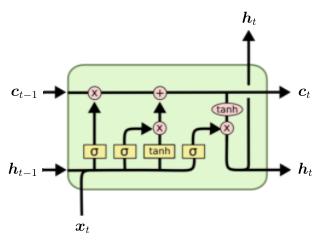
\includegraphics[width=.5\textwidth]{img/lstm_visual}
  \caption{Architecture of a single LSTM cell \cite{olah2015}. Trainable matrix multiplication followed by an activation function are in yellow boxes, and element-wise operations without learned parameters are in red ovals.}
  \label{fig:lstm_visual}
\end{figure}

The architecture of an LSTM is visualized in Figure \ref{fig:lstm_visual}. The forget vector acts as a gate which allows/disallows past information to persist over time, while the update and add vector grabs the data from the current input which is worth updating and remembering.


\subsection{Transformers and Attention}
Though LSTM networks presented a significant breakthrough in natural language processing (NLP), they have been quickly surpassed in the application of language modeling by attention-based methods. These models forgo the recurrent structure of information flow seen in RNN and LSTM for feed-forward layers and similarity scores between time steps. For example, calculating a similarity score between each pair of words in a sentence can help extract deeper context in language models such as transformers \cite{vaswani2017}.

While transformers are large neural networks with many components and parameters, they lean heavily on the attention mechanism. Given a $d$-dimensional feature vector $\vect x_t$ at each time-step $1\leq t\leq T$, define three trainable matrices $W_q$, $W_k$, and $W_v$. These are used to obtain a \textit{query}, \textit{key}, and \textit{value} vectors $\vect q_t$, $\vect k_t$, and $\vect v_t$ for each time-step. Note that these can be arranged into matrices $Q,K,V \in \R^{T\times d}$. Calculated the correlation between observation $t$ and all other time-steps:
\begin{equation}
  \vect c_t = \text{softmax}\left(\frac{K \vect q_t}{\sqrt{d}} \right) \in \R^T
  \label{eq:attn_cor}
\end{equation}


Notice that the matrix multiplication $K \vect q_t$ in Equation \ref{eq:attn_cor} is simply $T$ individual dot-product computations. So the $i$-th entry of $\vect c_t$ gives the similarity between the input at time $t$ and the input at time $i$. The softmax function $\text{softmax}(z_i) = \frac{e^{z_i}}{\sum_{j=1}^T e^{z_j}}$ rescales the dot product calculations so that the sum of the entries of $\vect c_t$ is equal to 1. In applications where an input $\vect x_{t_1}$ is not allowed to see information of future inputs $\vect x_{t_2}$, $t_1<t_2$, the corresponding entries of $K\vect q_{t_1}$ are masked to be $-\infty$. This causes the entries $c_{ti} = 0$ when $i > t$.

Next, the attention is calculated as 
\begin{equation}
  \vect a_t = V \vect c_t \in \R^d
  \label{eq:attn}
\end{equation}
The attention vector $\vect a_t$ is a weighted sum of the value vectors of each other time-step, weighted by the correlation scores in Equation \ref{eq:attn_cor}. The attention calculation can also be written more generally:
\begin{equation}
  A = \text{softmax}\left(\frac{QK^\top}{\sqrt{d}} \right) V \in \R^{T \times d}
  \label{eq:attn_matrix}
\end{equation}

In attention networks, the attention vectors $\vect a_t$ are individually sent through feed-forward layers. For example, transformers calculate attention and then use three feed-forward layers in a single ``block'' \cite{vaswani2017}. These blocks are stacked on top of each other up to six times to obtain deeper and deeper contextualization of the input sequence \cite{dai2019}. Eventually, this contextualization is plugged into a final prediction layer, depending on the application.

It should be pointed out that transformers and attention networks were developed for the NLP application. So in this case, a sequence of $T$ inputs represents a sentence of length $\leq T$ and an input vector $\vect x_t$ is a $d$-dimensional learned representation of an individual word \cite{mikolov2013}. Then the correlation score in Equation \ref{eq:attn_cor} is quantifying the relationship between pairs of words in the sentence.


